\chapter{Dise'no}\label{cap:dise'no}

	En este capítulo se expone de manera detallada el dise'no del sistema de actuaci'on y se analiza cada uno de los subsistemas que lo componen. El diseño se ha hecho teniendo en cuenta los requisitos indicados en el apartado \ref{sec:obj} del capítulo \ref{cap:intro}. 

\section{Descripci'on del sistema completo}\label{sec:arq_actuador}

	La arquitectura elegida se basa en un sistema de control en lazo cerrado, ya que hace al sistema m'as inmune frente a las perturbaciones y logra unos mejores ajustes. No se ha escogido la configuración en lazo abierto porque requiere de unos ajustes más precisos y es más sensible a las perturbaciones. Además, la temperatura de la sala depende de factores como el aislamiento de la sala, la temperatura exterior, el calor generado por los equipos, etc, cuyo impacto en la respuesta global es difícil de caracterizar con exactitud. En la figura \ref{4_1:diag_completo} se muestra un esquema de la arquitectura. 

\begin{figure}[htbp]
  \centering
  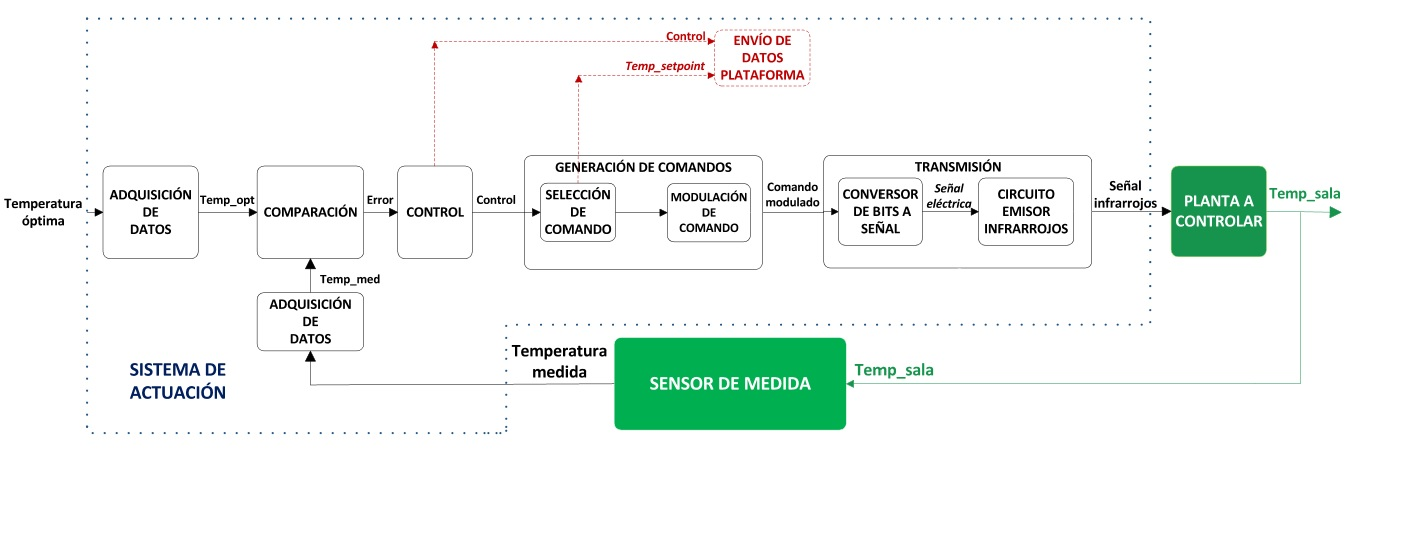
\includegraphics[width=95mm, height=220mm]{imagenes/capitulo4/4_1Diagrama_Completo}
   \caption{Diagrama del sistema completo}
   \label{4_1:diag_completo}
\end{figure}

	El sistema de actuaci'on tiene 2 entradas: la temperatura a la que debe estar la sala o \textit{temperatura 'optima}, proporcionada por el sistema de optimización y la temperatura a la que se encuentra la sala o \textit{temperatura medida},  proporcionada por el sensor. El sistema tiene una única salida que es el \textit{setpoint} del aire acondicionado. El sistema est'a formado por los siguiente bloques:
\begin{itemize}
    	\item Bloque de adquisici'on de datos.
    	\item Bloque de comparaci'on.
    	\item Bloque de control.
    	\item Bloque de generaci'on del comando.
    	\item Bloque de transimisi'on.
\end{itemize}

	En la figura \ref{4_1:diag_completo} tambi'en se incluyen la planta a controlar y el sensor de medida. Estos componentes son fundamentales para explicar el funcionamiento del actuador pero no forman parte de él, por lo que no son considerados en la etapa de dise'no. 

	Tambi'en existe un bloque de env'io de datos que se utiliza para mandar datos a la plataforma de monitorización y poder visualizar y evaluar el correcto funcionamiento del actuador. Este bloque se incluye en el dise'no, aunque no es fundamental para el funcionamiento del actuador.

	En los siguientes apartados se hace una descripci'on detallada de cada uno de los bloques del actuador.

\section{Bloque de adquisici'on de datos}\label{sec:adquisicion}

	Es la primera etapa del sistema de actuaci'on. El dato de \textit{temperatura 'optima} y el dato de \textit{temperatura medida} se encuentran almacenados en una plataforma y con un determinado formato. Hay que tener en cuenta el tipo de plataforma y el formato utilizado, ya que ambos varían seg'un el CPD e incluso puede darse el caso de que ambos datos est'en almacenados en plataformas diferentes y con distintos formatos. Tambi'en hay que considerar que el dato puede estar almacenado con un formato que no permite al actuador utilizarlo directamente y necesita ser procesado.

	El actuador va a disponer de 2 bloques de adquisici'on, uno para cada dato. Cada bloque tendr'a como entrada el dato de temperatura almacenado en la plataforma y como salida ese mismo dato procesado para que el actuador pueda utilizarlo. En la figura \ref{4_2:diag_adquisicion} se muestra un esquema de cada uno de estos bloques.	

\begin{figure}[htbp]
  \centering
  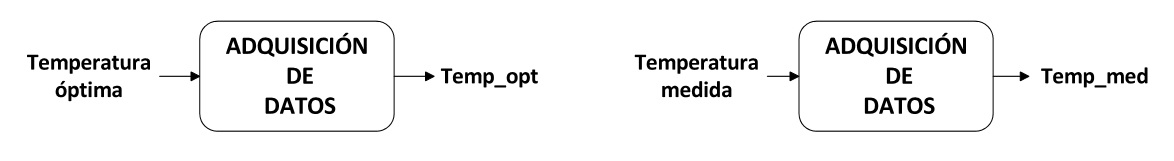
\includegraphics[width=142mm,height=20mm]{imagenes/capitulo4/4_2Bloque_Adquisicion}
   \caption{Esquema del bloque de adquisici'on de datos}
   \label{4_2:diag_adquisicion}
\end{figure}

	Para este trabajo se va a usar \textit{Graphite} como plataforma de almacenamiento de datos debido a que los sensores de la sala B039 env'ian los datos a un servidor que utiliza dicha plataforma. Según su documentación \cite{Graphite1}, \textit{Graphite} almacena series de datos junto con su marca temporal o \textit{timestamp}. Adem'as, proporciona una aplicaci'on web a trav'es de la cual se pueden visualizar los datos de forma gr'afica o se pueden exportar en diferentes formatos. En la figura \ref{4_3:interfaz_graphite} se muestra una imagen de la interfaz gr'afica de \textit{Graphite}.

\begin{figure}[htbp]
  \centering
  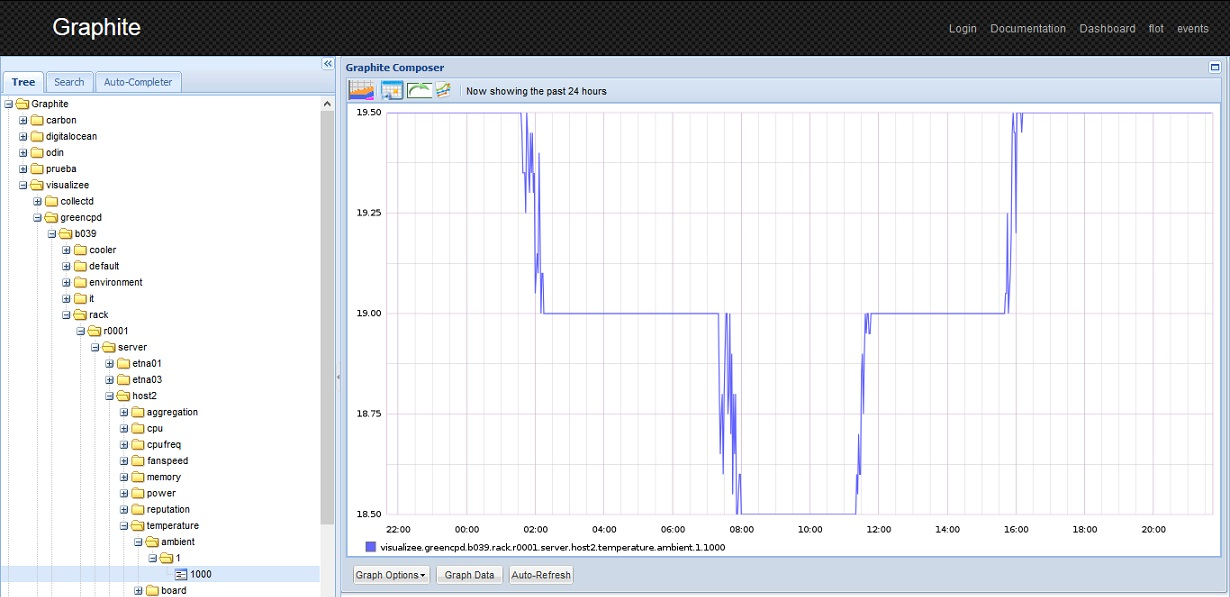
\includegraphics[width=140mm, height=75mm]{imagenes/capitulo4/4_3Interfaz_Graphite}
   \caption{Interfaz gr'afica de \textit{Graphite}}
   \label{4_3:interfaz_graphite}
\end{figure}

	\textit{Graphite} permite exportar los datos que tiene almacenados, en diferentes formatos. De entre todos ellos, se ha decidido utilizar JSON. El motivo es que tiene un esquema de representación fácil de entender y el procesamiento del dato es más fácil de hacer en este formato que en el resto de formatos existentes. A continuación se muestra un ejemplo de un dato que ha sido exportado de \textit{Graphite} en formato JSON:

\begin{verbatim}
   [{"target":visualizee.greencpd.rack.b039.cooler.temperature.supply.
   setpoint.2, "datapoints": [[18.0, 1496395200], [18.0, 1496395210], 
   [19.0, 1496395220], [21.0, 1496395230], [23.0, 1496395240], 
   [22.0, 1496395250]]}]
\end{verbatim}

	El objeto JSON posee 2 campos: \textbf{target} y \textbf{datapoints}. El campo \textbf{target} almacena una cadena de caracteres con la ruta en la que se encuentra el dato que se quiere exportar. El campo \textbf{datapoints} es un array de N-duplas donde cada dupla contiene el valor de la temperatura junto con el instante de medida o \textit{timestamp}. El valor de la temperatura es un n'umero real con una precisi'on de cent'esimas y el \textit{timestamp} es un entero que expresa el tiempo en formato epoch.

	Los datos almacenados en \textit{Graphite} se pueden exportar realizando una petici'on http. A continuaci'on se muestra un ejemplo del formato de una url usada para exportar un dato de la plataforma.

\begin{verbatim}
http://visualizee.die.upm.es:8000/render?format=json&target=visualizee.
.greencpd.b039.rack.r0001.server.host2.temperature.ambient.1.1000
&from=-1min&until=-4min
\end{verbatim}

	 Según la documentación \cite{Graphite1}, la url contiene 4 par'ametros que son configurados para seleccionar el dato que se desea exportar, el formato en el que se obtienen los datos y el número de muestras que se van a exportar. Estos par'ametros son:

\begin{itemize}
\item \textbf{format:} contiene el formato en el que se desea extraer los datos.
\item \textbf{target:} contiene la ruta donde se encuentra el dato a exportar.
\item \textbf{from:} contiene el instante de inicio de la toma de muestras. Si no se especifica nada, se toma por defecto las 'ultimas 24 horas. 
\item \textbf{until:} contiene el instante final de la toma de muestras. Si no se especifica nada, se toma por defecto el instante actual.
\end{itemize}

	En cada petición es recomendable exportar varias muestras y no sólo la del instante de la iteración, ya que puede darse el caso de que el sistema de actuación haga la petición del dato de temperatura y el sensor todavía no lo haya medido o genere null. De este modo, se soluciona este problema y el error cometido es mínimo porque la temperatura es una variable que evoluciona lentamente y la variación que puede producirse entre muestras muy próximas es muy pequeña. En este trabajo, el sensor de banco de pruebas toma muestras cada 10 segundos, luego se van a exportar las muestras de \textit{temperatura óptima} y \textit{temperatura medida} tomadas en el último minuto para tener un cierto margen de seguridad.

	Por 'ulltimo, una vez exportado el dato de la plataforma y extraído del objeto JSON, éste se multiplica por un factor de conversi'on para convertirlo a un número entero que tenga la precisión necesaria para ser utilizado en las siguientes etapas. En este trabajo, el bloque de comparación y de control van manejar números enteros que representan a números reales con una precisión de milésimas. Por tanto, el factor de conversión es 1000. De este modo, se conserva la precisión del dato de temperatura y ya está preparado para ser usado en próximas etapas.

\section{Bloque de comparaci'on}\label{sec:comparacion}

Su función es calcular el error que hay entre la \textit{temperatura 'optima} y la \textit{temperatura medida}. En la figura \ref{4_4:diag_comparacion} se muestra un diagrama de este bloque. 

\begin{figure}[htbp]
  \centering
  \includegraphics[width=100mm, height=25mm]{imagenes/capitulo4/4_4_Bloque_Comparacion}
   \caption{Diagrama del bloque de comparaci'on}
   \label{4_4:diag_comparacion}
\end{figure}

	El bloque resta a la \textit{temperatura óptima} el valor de la \textit{temperatura medida}. El resultado de dicha operación es el valor de la señal de error. El error está expresado en las mismas unidades que las temperaturas.

\section{Bloque de control}\label{sec:control}

	Su función es generar la señal de control que se enviará al sistema de refrigeración para que la sala alcance la \textit{temperatura óptima}. Dicha señal es generada a partir de la señal de error y siguiendo un determinado algoritmo o pol'itica de control. En la figura \ref{4_5:diag_control} se muestra un esquema con las entradas y salidas del bloque.

\begin{figure}[htbp]
  \centering
  \includegraphics[width=100mm, height=22mm]{imagenes/capitulo4/4_5_Bloque_Control}
   \caption{Esquema del bloque de control}
   \label{4_5:diag_control}
\end{figure}

	De todos los controladores explicados en el capítulo \ref{cap:estadoarte}, se ha escogido el controlador PID, ya que es un controlador ampliamente usado en la industria, incluyendo procesos de control de la temperatura, con un planteamiento sencillo y con diferentes métodos de diseño y ajuste. Se ha decidido usar la representación ideal o paralela.

	El ajuste del controlador puede realizarse tanto en el dominio del tiempo como en la frecuencia \cite{PID}. Algunos de los métodos utilizados son: Ziegler-Nichols, diagrama de bode, criterio de Routh-Hurwitz, lugar de raíces, método de prueba y error... 

	Algunos de estos métodos permiten el ajuste de la planta sin necesidad de conocer su función de transferencia. Sin embargo, es recomendable obtener dicha función, para así facilitar el proceso de ajuste de los parámetros. Por otro lado, la expresi'on anterior está definida para un controlador en tiempo continuo. Sin embargo, el controlador se va a implementar en un sistema digital, luego es necesario discretizarlo. 

	Por tanto, el proceso de diseño del controlador consta de las siguientes fases: primero, se estima la función de transferencia que modela la planta a controlar. Después, se diseña el controlador PID y se ajustan sus parámetros usando alguno de los métodos anteriormente descritos. Por último, se discretiza el controlador PID diseñado. A continuación, se explican cada una de estas fases en los siguientes apartados.

\subsection{Caracterizaci'on de la planta}\label{subsec:caract_planta}

	En esta fase se va a estimar la función de transferencia que representa el comportamiento dinámico de la planta. La variable a controlar es la temperatura de la sala y dicho control se va a realizar a trav'es del sistema de refrigeraci'on de la sala. Por tanto, la planta a controlar está formada por el sistema de refrigeraci'on y la sala. 

	La planta puede ser caracterizada aplicando modelos f'isicos de los distintos componentes que componen la planta (ciclo de refrigeración + sala). Sin embargo, esto es poco viable porque hay par'ametros que son dif'iciles de caracterizar y medir. 

	Por este raz'on, se decide hacer la caracterizaci'on de la sala mediante la t'ecnica de identificaci'on de sistemas. Se van a realizar una serie de experimentos basados en excitar la planta con una se'nal de entrada específica (escalón, rampa...) y se miden los valores generados en la salida. Despu'es, se aplican m'etodos estad'isticos que permiten estimar una funci'on matem'atica que representa el comportamiento de la planta. 

	El experimento realizado en este trabajo se basa en aplicar una se'nal de entrada de tipo escal'on al sistema de refrigeraci'on y medir la temperatura de la sala. El valor inicial y el valor final de la señal escalón son el valor mínimo y máximo de funcionamiento del sistema de refrigeración (18{$^{\circ}$}C y 32{$^{\circ}$}C respectivamente). De este modo,se pretende abarcar todo el rango de  de funcionamiento del sistema de refrigeración y caracterizar mejor la planta. 

	Hay que tener en cuenta que aunque la temperatura máxima sea de 32{$^{\circ}$}C, la sala no puede alcanzar ese valor, ya que la temperatura máxima recomendada para el buen funcionamiento de la sala está entre (25{$^{\circ}$}C - 27{$^{\circ}$}C) y si se supera, podrían dañarse los equipos. Por tanto, el experimento se mantendrá hasta que la sala alcance ese valor recomendado. 

	Los valores de la salida son medidos cada 10 segundos, ya que es el periodo de muestreo del sensor. Podr'ia haberse elegido un periodo de muestreo superior, por ejemplo 1 min, ya que la evoluci'on de la temperatura es un proceso lento. Sin embargo, se opta por un periodo igual al periodo de muestreo del sensor y se evita tener que hacer un procesamiento adicional. Este experimento se repetirá varias veces para obtener un mayor n'umero de muestras.

	Una vez realizados todos los experimentos, se estima la funci'on transferencia de la planta, utilizando el programa de c'alculo matem'atico MATLAB. Se va a dise'nar un script con el que se obtiene los valores de la se'nal de entrada y de salida utilizadas en cada experimento. Después se estima la función de transferencia usando la funci'on de matlab \textit{tfest}. Esta funci'on toma como par'ametros los datos de entrada y de salida y el n'umero de polos y ceros del sistema. Para cada conjunto de datos se van a realizar todas las combinaciones posibles de polos y ceros hasta orden 3, ya que este tipo de sistemas suelen ser de 1{$^{\circ}$}o 2{$^{\circ}$} orden y no es recomendable usar sistemas cuyo orden es muy elevado debido al problema de sobreajuste u \textit{overfitting}. El objetivo es estimar una función que tenga un buen ajuste con cualquier conjunto de datos.

	Una vez se han obtenido todas las combinaciones, se escoge aquella que tenga un mejor coeficiente de ajuste. Este coeficiente de ajuste es proporcionado por la misma función \textit{tfest} y es calculado mediante el error cuadr'atico medio normalizado o NRMSE \textit{Normalized Root-Mean-Square Error}. 

	La función \textit{tfest} presenta el inconveniente de que sólo puede manejar un conjunto de datos a la vez, por lo que no se puede calcular una estimación basada en los conjuntos de datos de todos los experimentos. Para solucionar este problema, se calcula el coeficiente de ajuste que tiene cada funci'on de transferencia de cada experimento, con respecto a sus datos y a los datos de los otros experimentos y se calcula el valor medio. Con esta información se selecciona la función que presente un mejor ajuste tanto a sus datos como a los datos del resto de experimentos.

	En caso de que hubiera varios experimentos con un coeficiente de ajuste medio parecido, se calcula también el error medio y el m'aximo error absoluto y se representa cada parámetro junto con el coeficiente de ajuste en un diagrama de pareto para decidir mejor cuál de ellas se ajusta mejor.

	Este proceso de caracterización descrito, en principio puede ser aplicado a otros bancos de pruebas, siempre y cuando sea adaptado a sus características particulares. 

	Por claridad, en este apartado sólo se muestra la función escogida. En el anexo \ref{ftrans} se detallan todas las  funciones de transferencia de todos los experimentos, así como el proceso de selección de la función de transferencia. A continuación se muestra la función de transferencia que caracteriza a la planta.

\begin{equation}\label{ecuacion4_2}
          \normalsize G(s) = \frac{8,4315 \cdot 10^{-5}s + 1,6968 \cdot 10^{-9}}{s^{3} + 0,2820s^{2} + 2,1553\cdot 10^{-4}s + 1,0462\cdot10^{-14}}
\end{equation} 

\subsection{Dise'no del controlador PID}\label{subsec:diseñoPID}

	El diseño del controlador consiste en ajustar los parámetros  $K_{p}$, $K_{i}$ y $K_{d}$ para que la respuesta cumpla una serie de especificaciones. El controlador que se va a diseñar debe cumplir las siguientes especificaciones.

\begin{itemize}
	\item El sistema debe ser estable en todo momento.
	\item El error estacionario para una señal escalón debe ser próximo a cero con una tolerancia del 5\%.
	\item El tiempo de establecimiento del sistema debe ser menor de 10 min. Este requisito puede verse incumplido debido a las limitaciones físicas. La temperatura tiene una evolución lenta y no puede fijarse un tiempo de establecimiento pequeño.
\end{itemize}

	Para ajustar los parámetros del controlador se decidió inicialmente usar el método de Ziegler-Nichols \cite{PID}. Este método posee 2 versiones que permiten ajustar el sistema dependiendo de si la planta tiene una respuesta con forma de \textit{ese} o posee una respuesta con oscilaciones para una determinada ganancia $K_{cr}$. 

	La función estimada no cumplía los requisitos para aplicar la 2º versión, por lo que se decidió aplicar la 1º versión. Aunque la respuesta de la planta en lazo abierto era estable, no presentaba dicha forma, por lo que resultaba complicado aplicar este método y también fue descartado. También se decidió probar otros métodos como el diagrama de bode pero al tener un margen de ganancia infinito y un margen de fase elevado resultaba complicado establecer un patrón para realizar el ajuste.

	Por tanto, se ha decidido escoger el método de ajuste y error. Este método consiste en ir ajustando los parámetros del controlador PID hasta conseguir que se cumplan las especificaciones fijadas. El proceso llevado a cabo es el siguiente:

\begin{enumerate}
	\item Se fijan los valores de $ K_{i}$ y $K_{d}$ al valor más pequeño posible y se fija la constante proporcional a 1. Se va incrementando dicha ganancia hasta conseguir oscilaciones estables y próximas al valor deseado.
	\item Se incrementa el valor de $K_{i}$ hasta conseguir eliminar el error estacionario. Si es necesario, se disminuye ligeramente el valor $K_{p}$ para eliminar las oscilaciones.  
	\item Se incrementa el valor de $K_{d}$ hasta conseguir la respuesta deseada pero más rápida. Si es necesario, se aumenta ligeramente el valor de $K_{p}$.
\end{enumerate}

	El proceso de ajuste de los parámetros del controlador y la simulación de la respuesta del sistema se ha realizado a través de MATLAB. Se ha diseñado un script que simula el sistema de control en lazo cerrado formado por el controlador PID y la función de transferencia de la planta a controlar. Este script genera la respuesta del sistema de control en base a los parámetros del PID y permite evaluar la estabilidad del sistema mediante el diagrama de Nyquist.  En el anexo \ref{Anexo:scriptPID} puede verse el script elaborado.

	A continuación se muestra en la figura \ref{4_6:resp_simulacion} una imagen con la respuesta obtenida en la simulación. Los valores de $K_{p}$, $K_{i}$ y $ K_{d}$ que cumplen con las especificaciones son:
\begin{align*}
	K_{p} &= 28; \quad K_{i}=0.037; \quad K_{d}= 300;
\end{align*}

\begin{figure}[H]
  \centering
  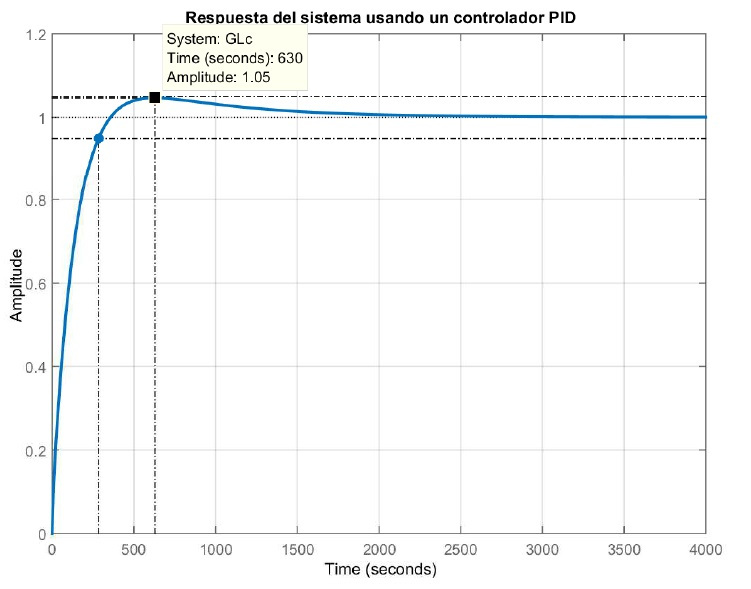
\includegraphics[width=110mm, height=80mm]{imagenes/capitulo4/4_6Resp_Lazo_Cerrado}
   \caption{Respuesta del sistema a una entrada escalón usando el PID diseñado}
   \label{4_6:resp_simulacion}
\end{figure}

\subsection{Discretizaci'on del controlador PID}\label{subsec:discretizacionPID}

	La discretización del controlador PID consiste en obtener la expresión matemática del controlador PID en tiempo discreto para que pueda ser implementado en un sistema digital. Para ello, se va a discretizar cada una de las acciones que definen al controlador PID y se agrupan las expresiones obtenidas en cada discretización. A continuación se detalla la discretización de cada acción:

\begin{itemize}
         \item\textbf{Discretizaci'on de la acci'on proporcional:} es la m'as f'acil de realizar ya que se basa en el muestreo de la se'nal de error.
	\begin{equation}\label{ecuacion_prop}
		\large m_{p}(n) =\left. K_{p} e(t) \right|_{t=kT_{s}} =  K_{p} e(kT_{s}) =   K_{p} e(n)
           \end{equation}
	\item\textbf{Discretizaci'on de la acci'on integral:} se basa en la discretizaci'on de la integral. Existen diferentes m'etodos para poder discretizarla (integraci'on hacia delante, integraci'on hacia atr'as, m'etodo de tustin...)\cite{PID}. Se ha decidido escoger el m'etodo de tustin ya que es una aproximaci'on m'as precisa y permite conservar la estabilidad del sistema en tiempo discreto.
	\begin{equation}\label{ecuacion_int}
	   \begin{split}
		 m_{i}(n) & = \left.  K_{i}\int_0^t e(t)dt \right|_{t=kT_{s}} =  K_{i}\sum_{k=1}^n  T_{s}\frac{e(kT_{s}) + e([k+1]T_{s})}{2} \\
                                     & = m_{i}(n-1) +  T_{s}\frac{e(kT_{s}) + e( [k+1]T_{s}\big)}{2} 
 	   \end{split}	
	\end{equation}
	 \item \textbf{Discretizaci'on de la acción derivativa:} se basa en la aplicaci'on del m'etodo de Euler hacia atr'as. De este modo, se consigue conservar la estabilidad.
            \begin{equation}\label{ecuacion_der}
		m_{d}(n)  =\left.  K_{d} \frac{de(t)}{dt} \right|_{t=kT_{s}}= K_{d} \frac{e(kT_{s}) - e([k-1]T_{s})}{T_{s}}
	\end{equation}
\end{itemize}

	Por tanto, la se'nal de control en el instante \textit{n} es la suma de las ecuaciones \ref{ecuacion_prop}, \ref{ecuacion_int} y \ref{ecuacion_der}. Para obtener una expresión más simplificada y fácil de implementar, se calcula la expresión de señal de control en \textit{n-1} y se hace la resta de la expresión en \textit{n} con la de \textit{n-1}. La expresión obtenida es la siguiente:
\begin{equation}\label{ecuacion4_6}
		m(n) = m(n-1) + q_{0} e(n) + q_{1} e(n-1) + q_{2} e(n-2)   
\end{equation}
	donde los coeficientes {$q_{0}$, $q_{1}$  y $q_{2}$ tienen las siguientes expresiones:\\
\begin{equation}\label{ecuacion4_7}
		q_{0} = \left( K_{p} + \frac{K_{d}}{T_{s}} +  \frac{K_{i}T_{s}}{2} \right) \quad q_{1} = \left( - K_{p} - \frac{2K_{d}}{T_{s}} +  \frac{K_{i}T_{s}}{2} \right)  \quad q_{2} = \frac{K_{d}}{T_{s}}
\end{equation}

	Para verificar que la discretización es válida, se ha simulado en MATLAB dicha discretización y se ha comparado con la respuesta de la figura \ref{4_6:resp_simulacion}. Dicha comparativa puede verse en figura \ref{4_7:discretizacionPID}. En dicha imagen se observa que la discretización se aproxima con bastante precisión a la respuesta continua.

\begin{figure}[h]
  \centering
  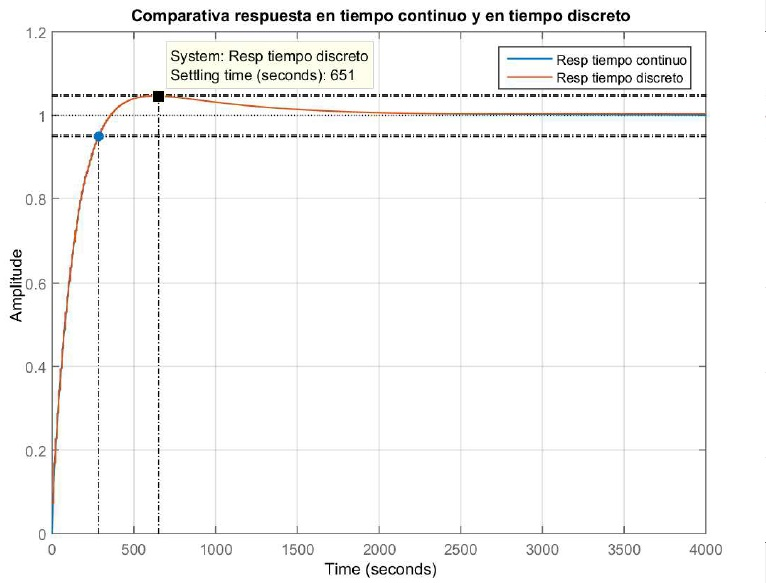
\includegraphics[width=110mm, height=71mm]{imagenes/capitulo4/4_7Resp_Lazo_Cerrado_Discreto}
   \caption{Respuesta del sistema a una entrada escalón con el PID discretizado}
   \label{4_7:discretizacionPID}
\end{figure}

\section{Bloque de generación de comandos}\label{sec:comandos}

	Este bloque se ha dividido en 2 subbloques para facilitar la implementación y modularidad. En la figura \ref{4_8:diag_generacion_comandos} se muestra un esquema de las entradas y salidas del bloque y los subbloques que lo componen.

\begin{figure}[htbp]
  \centering
  \includegraphics[width=100mm, height=26mm]{imagenes/capitulo4/4_8_Generacion_Comandos}
   \caption{Esquema del bloque de generaci'on de comandos}
   \label{4_8:diag_generacion_comandos}
\end{figure}

	El subbloque de \textbf{selección del comando} selecciona el \textit{setpoint}, a partir del valor de la se'nal de control y el rango de funcionamiento del sistema de refrigeraci'on, y selecciona el comando asociado. El subbloque de \textbf{modulación del comando} modula ese comando para que pueda ser interpretado por el sistema de refrigeraci'on. 

\subsection{Subbloque de selecci'on del comando}\label{subsec:seleccionComando}

Su función es seleccionar la temperatura del sistema de refrigeraci'on a partir del valor de señal de control y teniendo en cuenta el rango de valores de funcionamiento. Dicho rango es un conjunto finito de valores discretos con una separación fija entre valores consecutivos. Teniendo en cuenta esto, se va a aplicar el siguiente criterio para seleccionar la temperatura:

\begin{itemize}
\item\textbf{Se'nal de control igual o superior a la temperatura m'axima:} en este caso se escoge la temperatura m'axima de funcionamiento. 
\item\textbf{Se'nal de control entre la temperatura m'inima y m'axima:} se escoge la temperatura obtenida del resultado de redondear el valor de la se'nal de control al entero m'as pr'oximo.
\item\textbf{Se'nal de control igual o inferior a la temperatura m'inima:} en este caso se escoge la temperatura m'inima de funcionamiento. 
\end{itemize}

	Hay que tener en cuenta que el valor de la señal de control est'a expresado en mil'esimas, por lo que es necesario convertirlo a unidades para poder seleccionar la temperatura de forma adecuada.

	Después, una vez fijada la temperatura de funcionamiento, se selecciona el comando asociado a esa temperatura. Un comando es una secuencia de bits (0's y 1's) que representa un modo de funcionamiento que puede ejecutar el sistema de refrigeraci'on. 

	Hace unos a'nos, algunos miembros de \textit{GreenLSI} realizaron un proyecto denominado Pimote \cite{PIMOTE}. Este proyecto consist'ia en el dise'no e implementaci'on de un mando a distancia universal. En ese trabajo se utiliz'o como banco de pruebas el sistema de refrigeraci'on de la sala B039, que es el mismo que se utiliza en este trabajo, por lo que están disponibles sus comandos de funcionamiento. Cada uno de estos comandos est'a almacenado en un fichero de texto y siguiendo un determinado protocolo. 

	Se ha decicido utilizar los comandos usados en el proyecto Pimote y el protocolo que utilizan. Dicho protocolo es sencillo y en él están perfectamente delimitados cada uno de los campos que componen el comando. La única modificación que se va a hacer en este trabajo es convertir cada fichero a formato binario para facilitar su uso en el sistema de actuación.  En la figura \ref{4_9:protocolo_comando} se muestra el esquema del protocolo. 
\begin{figure}[h]
  \centering
  \includegraphics[width=140mm, height=18mm]{imagenes/capitulo4/4_9_Protocolo_Comandos}
   \caption{Protocolo de almacenamiento del comando}
   \label{4_9:protocolo_comando}
\end{figure}

\noindent A continuación se detallan cada uno de los campos del protocolo:

\begin{itemize}
     \item\textbf{Bytes de relleno:} son 6 bytes y est'an reservados por si fuera necesario incluir un campo nuevo en la cabecera o ampliar el tama'no de un campo ya definido.
     \item\textbf{Longitud del Payload:} est'a formado por 1 byte e indica el n'umero de bytes que ocupa el campo de datos del comando.
      \item\textbf{Periodo de bit:} est'a formado por 2 bytes y contiene el tiempo de bit del comando expresado en microsegundos.
      \item\textbf{Periodo de la portadora:} est'a formado por 1 byte y contiene el periodo de la portadora expresado en microsegundos. 
      \item\textbf{Payload:} su tamaño varía según el comando seleccionado. Contiene la orden o modo de funcionamiento del aire acondicionado.
\end{itemize}

\subsection{Subbloque de modulaci'on del comando}\label{subsec:modulacion}

	Se función es modular el comando que se envía al aire acondicionado para que el receptor pueda interpretarlo y ejecutar la orden. En este trabajo se va a usar una modulaci'on digital de amplitud usando como portadora una se'nal cuadrada de periodo T\_carrier. En la figura \ref{4_10:modulacion_bits} se muestra un esquema que representa la modulaci'on de la secuencia de bits `0101'.  A continuaci'on se describe el proceso de modulaci'on de cada bit: 

\begin{itemize}
    \item\textbf{Modulaci'on de un `1':} se transmite una se'nal cuadrada de frecuencia igual a la portadora y durante un tiempo igual al periodo de bit . 
    \item\textbf{Modulaci'on de un `0':} no se transmite nignuna se'nal durante un tiempo igual al periodo de bit. 
\end{itemize}

\begin{figure}[htbp]
  \centering
  \includegraphics[width=100mm, height=35mm]{imagenes/capitulo4/4_10_Modulacion_Bits}
   \caption{Ejemplo de modulaci'on de una secuencia de bits 0101}
   \label{4_10:modulacion_bits}
\end{figure}


\section{Bloque de transmisi'on}\label{sec:transmision}

	Su función es enviar el comando al sistema de refrigeraci'on. Para facilitar su implementación y modularidad, se ha dividido en 2 subbloques. En la figura \ref{4_11:diag_transmision} se muetra un esquema con sus entradas y salidas, así como de los subbloques que lo componen. 

\begin{figure}[htbp]
  \centering
  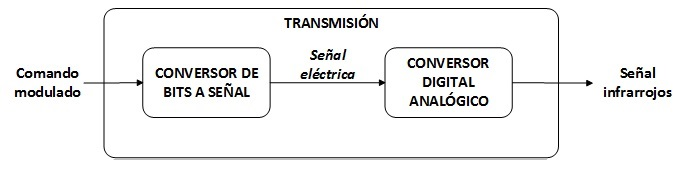
\includegraphics[width=140mm, height=32mm]{imagenes/capitulo4/4_11Bloque_Transmision}
   \caption{Diagrama del bloque de transmisi'on}
   \label{4_11:diag_transmision}
\end{figure}

	Primero, el \textbf{conversor de bits a señal} genera una señal eléctrica a partir de la secuencia de bits del comando y posteriormente, el \textbf{el circuito emisor de infrarrojos} la convierte en una señal de infrarrojos para que el sistema de refrigeración pueda interpretarla. A continuación se explican ambos subbloques con más detalle.

\subsection{Conversor de bits a señal}\label{subsec:conversor}

	Convierte la secuencia de bits que representa el comando modulado, en una se'nal el'ectrica. Dicha se'nal debe cumplir los requisitos de tiempo definidos en la modulaci'on (periodo de bit y periodo de la portadora). La transmisi'on de cada bit debe hacerse de forma síncrona para controlar el tiempo de bit y el tiempo de portadora. 

	Para ello, se ha decidido utilizar el protocolo SPI \textit{Serial Peripheral Interface}\cite{SPI}. Es un protocolo de comunicación serie síncrono que permite la transferencia de información entre un nodo principal llamado \textit{nodo maestro} y uno o varios nodos secundarios llamados \textit{nodos esclavos}. La transmisión de la información se realiza byte a byte, con un bit de parada entre transmisiones consecutivas. Un dispositivo SPI está formado por 4 pines:

\begin{itemize}
   \item\textbf{MOSI:} pin que se utiliza para enviar informaci'on a los nodos esclavos.
   \item\textbf{MISO:} pin que se utiliza para recibir informaci'on de los nodos esclavos. 
   \item\textbf{SCLK:} pin que emite una señal de reloj cuadrada, de frecuencia configurable, que se utiliza para sincronizar el envío de información entre los nodos.
   \item\textbf{CE:} pin que se utiliza para habilitar o deshabilitar la comunicaci'on con los nodos esclavos.
\end{itemize}

	La elecci'on de este protocolo se debe a que se puede controlar el tiempo de duraci'on de cada bit a trav'es de la se'nal SCLK. Por tanto, se puede realizar la modulaci'on correctamente y cumpliendo los requisitos de periodo de bit y periodo de portadora fijados en la etapa de modulaci'on. La interfaz SPI emite una señal eléctrica por el pin MOSI cuando se desear enviar el bit `1' ~ y no emite nada cuando se desea enviar el bit `0'. EL bit `1' ~ se asocia con un nivel de tensión alto (3,3 V o 5V), mientras que el bit `0' ~  se asocia con un nivel de tensión próximo a 0V.

\subsection{Circuito emisor de infrarrojos}\label{subsec:infrarrojos}

	Convierte la señal eléctrica en una señal de infrarrojos y la emite al sistema de refrigeración. En la figura \ref{4_12:emisor_IR} puede verse el esquema del circuito.

\begin{figure}[htbp]
  \centering
  \includegraphics[width=70mm, height=42mm]{imagenes/capitulo4/4_12_Emisor_IR}
   \caption{Esquema del circuito emisor de infrarrojos}
   \label{4_12:emisor_IR}
\end{figure}

	El circuito se basa en un diodo LED de infrarrojos (IRLED), un transistor BJT y un conjunto de resistencias. La resistencia R1 se usa para obtener la corriente de base que permite al transistor entrar en la región de saturación y la resistencia R2 se usa para polarizar el diodo en su punto de trabajo. El transistor trabaja en saturación y corte para que el diodo pueda generar la señal a transmitir. 

	El funcionamiento del transistor es el siguiente: cuando no se recibe tensión en la entrada del circuito (equivale a un '0'), el transistor entra en corte y la corriente de base y colector son muy próximas a 0. Al no haber corriente de colector, no circula corriente por el diodo, luego no emite señal. Sin embargo, cuando se recibe un nivel de tensión en la entrada (equivale a un '1'), el transistor entra en la región de saturación y circula corriente a través del diodo. El diodo convierte esa corriente en una señal de infrarrojos y la emite al sistema de refrigeración.

\section{Bloque de envío de datos}\label{sec:envioDatos}

	La función de este bloque es subir datos a la plataforma \textit{Graphite}. En la figura \ref{4_13:envio_datos} se muestra un esquema de sus entradas y salidas.

\begin{figure}[htbp]
  \centering
  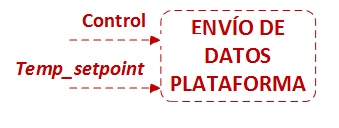
\includegraphics[width=70mm, height=30mm]{imagenes/capitulo4/4_13_Envio_Datos}
   \caption{Esquema del bloque de envío de datos}
   \label{4_13:envio_datos}
\end{figure}

	El bloque posee dos entradas, el dato de temperatura de control y el dato de \textit{setpoint}. Dichos valores se suben a la plataforma una vez se ha obtenido la temperatura de control y se ha seleccionado el \textit{setpoint}. El objetivo es poder visualizar el comportamiento de estas señales y así poder evaluar el comportamiento del actuador.

	Aunque no aparezca en el diagrama, en la fase de implementación se considerará la \textit{temperatura óptima} como otra entrada. El motivo es que en este trabajo  la \textit{temperatura óptima} va a estar fijada por el usuario y es necesario subir dicho valor a la plataforma. Una vez el actuador esté integrado con el sistema de optimización del CPD, dicho valor será leído desde la plataforma y no será necesario subirlo.

	Para poder subir los datos a la plataforma se ha tenido en cuenta los diferentes métodos disponibles para subir un dato, según  la documentación de \textit{Graphite} \cite{Graphite1}. Se ha usado un formato de texto plano para subir los datos, ya que presenta un formato sencillo y es fácil de implementar. Dicho formato presenta la estructura:

	\begin{verbatim}
	           <metric_path> <metric_value> <metric_timestamp>
	\end{verbatim}
 	
	El parámetro \textit{<metric\_path>} debe contener la dirección http y el puerto del servidor, junto con la ruta donde se va a escribir el dato. El parámetro \textit{<metric\_value>} debe contener el dato que se quiere subir a la plataforma. Por último, el parámetro \textit{<metric\_timestamp>} debe contener el instante de tiempo en el que se midió el dato.
